\chapter{1 ноября}

\section{Исследование статистической зависимости}

%<*32>
Требуется определить, как зависит наблюдаемая случайная величина от одной или нескольких других величин, причём необязательно все величины случайные. Хотелось бы построить математическую модель, которая будет с некоторой надежностью предсказывать значение искомой величины при известных прочих величинах.

\begin{remark}
    Предсказывать мы можем лишь \underline{среднее значение} наблюдаемых случайных величин.
\end{remark}

\subsection{Математическая модель регрессии}

Пусть случайная величина \(X\) зависит от случайной величины \(Z\). Значение \(Z\) мы либо наблюдаем, либо задаём.

\begin{definition}
    \textbf{Регрессией} \(X\) на \(Z\) называется функция \(f(z) = \E (X \mid Z = z)\). Она показывает зависимость среднего значения \(X\) от значения \(Z\).
\end{definition}

\begin{definition}
    Уравнение \(X = f(Z)\) называется \textbf{уравнением регрессии}, а её график --- \textbf{линией регрессии}.
\end{definition}

Пусть при \(n\) экспериментах при значениях \(z_1 \dots z_n\) случайной величины \(Z\) наблюдались значения \(X_1 \dots X_n\) случайной величины \(X\). Обозначим через \(\varepsilon_i\) разницу между экспериментальными и теоретическими значениями случайной величины \(X\):
\[\varepsilon_i = X_i - \E(X \mid Z = z_i) = X_i - f(z_i)\]
Тогда \(X_i = f(z_i) + \varepsilon_i, 1 \leq i \leq n\), и \(\varepsilon_i\) можно понимать, как ошибку эксперимента.

\begin{remark}
    Обычно можно считать, что \(\varepsilon_i\) --- независимая одинаковая нормальная случайная величина: \(\varepsilon_i \in N(0; \sigma^2)\). \(a = 0\), т.к.
    \[\E \varepsilon_i = \E (X_i) - \E(f(z_i)) = \E (X_i) - \E(X \mid Z = z_i) = 0\]
\end{remark}

\begin{remark}
    В реальности \(\varepsilon_i\) могут быть зависимыми, это явление называется автокорреляция, особенно часто проявляется во временных рядах.
\end{remark}

\textit{Цель:} по данным значениям \(z_1 \dots z_n\) и \(X_1 \dots X_n\) как можно более точно оценить функцию \(f(z)\).

\begin{remark}
    При этом предполагается (из теории), что \(f(z)\) --- функция определенного типа, параметры которой неизвестны.
\end{remark}

\subsubsection{Метод наименьших квадратов}

Метод наименьших квадратов состоит в выборе параметров функции \(f(z)\) таким образом, чтобы минимизировать сумму квадратов ошибок:
\[\sum_{i=1}^{n} \varepsilon_i^2 = \sum_{i=1}^{n} (X_i - f(z_i))^2 \to \min\]
\begin{definition}
    Пусть \(\theta = (\theta_1 \dots \theta_k)\) --- набор неизвестных параметров функции \(f(z)\). Оценка \(\hat{\theta}\), при которой достигается минимум суммы квадратов ошибок, называется \textbf{оценкой метода наименьших квадратов (ОМНК)}.
\end{definition}
%</32>

\subsubsection{Линейная парная регрессия}

%<*33>
Пусть имеется линейная регрессия \(f(z) = a + bz\). Тогда \(X_i = a + bz_i + \varepsilon_i, 1 \leq i \leq n\), найдём оценки неизвестных параметров \(a\) и \(b\) методом наименьших квадратов (МНК):
\[\sum_{i=1}^{n} \varepsilon_i^2 = \sum_{i=1}^{n} (X_i - a - bz_i)^2 \to \min\]
\begin{align*}
    0 = \frac{\partial}{\partial a} \sum_{i=1}^{n} \varepsilon_i^2
     & = 2 \sum_{i=1}^{n} (X_i - a - b z_i) \cdot ( - 1)                     \\
     & = - 2 \sum_{i=1}^{n} X_i + 2 \sum_{i=1}^{n} a + 2 \sum_{i=1}^{n} bz_i \\
     & = - 2 \left(n \overline{X} - na - b n\overline{Z}\right)
\end{align*}

\begin{align*}
    0 = \frac{\partial}{\partial b} \sum_{i=1}^{n} \varepsilon_i^2
     & = 2 \sum_{i=1}^{n} (X_i - a - b z_i) \cdot ( - z_i)                      \\
     & = - 2 \left(n \overline{XZ} - an \overline{Z} - b n\overline{Z^2}\right)
\end{align*}

\[\begin{cases}
        n \overline{X} - na - bn \overline{Z} = 0 \\
        n \overline{XZ} - na \overline{Z} - bn \overline{Z^2} = 0
    \end{cases}\]
\[\begin{cases}
        \overline{X} - a - b \overline{Z} = 0 \\
        \overline{XZ} - a \overline{Z} - b \overline{Z^2} = 0
    \end{cases}\]
\[\begin{cases}
        a + b \overline{Z} = \overline{X} \\
        a \overline{Z} + b \overline{Z^2} = \overline{XZ}
    \end{cases}\]
Система такого вида называется системой нормальных уравнений.

\[\begin{cases}
        a = \overline{X} - b \overline{Z} \\
        (\overline{X} - b \overline{Z}) \overline{Z} + b \overline{Z^2} = \overline{XZ}
    \end{cases}\]
\[\begin{cases}
        a = \overline{X} - b \overline{Z} \\
        b(\overline{Z^2} - \overline{Z}^2) = \overline{XZ} - \overline{X} \cdot \overline{Z}
    \end{cases}\]
\[\begin{cases}
        a = \overline{X} - b \overline{Z} \\
        b = \frac{ \overline{XZ} - \overline{X} \cdot \overline{Z}}{ \overline{Z^2} - \overline{Z}^2}
    \end{cases}\]
\[\begin{cases}
        a = \overline{X} - b \overline{Z} \\
        b = \frac{ \overline{XZ} - \overline{X} \cdot \overline{Z}}{ \hat{\sigma}_z^2}
    \end{cases}\]
, где \(\hat{\sigma}_z^2\) --- выборочная дисперсия \(Z\) (неисправленная).

Запишем уравнение линейной регрессии в удобном виде.
\begin{align*}
    \overline{X_z}                                       & \coloneqq \E (\overline{X} \mid Z = z) = f(z)                                                                                                              \\
    \overline{X_z}                                       & = a + bz                                                                                                                                                   \\
    \overline{X_z}                                       & = \overline{X} - b \overline{Z} + bz                                                                                                                       \\
    \overline{X_z} - \overline{X}                        & = - b \overline{Z} + bz                                                                                                                                    \\
    \overline{X_z} - \overline{X}                        & = b (z - \overline{Z})                                                                                                                                     \\
    \overline{X_z} - \overline{X}                        & = \frac{ \overline{XZ} - \overline{X} \cdot \overline{Z}}{ \hat{\sigma}_z^2} (z - \overline{Z})                                                            \\
    \overline{X_z} - \overline{X}                        & = \frac{ \overline{XZ} - \overline{X} \cdot \overline{Z}}{ \hat{\sigma}_z \hat{\sigma}_x} \cdot \frac{ \hat{\sigma}_x}{ \hat{\sigma}_z} (z - \overline{Z}) \\
    \frac{\overline{X_z} - \overline{X}}{\hat{\sigma}_x} & = \frac{ \overline{XZ} - \overline{X} \cdot \overline{Z}}{ \hat{\sigma}_z \hat{\sigma}_x} \cdot \frac{ z - \overline{Z}}{ \hat{\sigma}_z}                  \\
    \frac{\overline{X_z} - \overline{X}}{\hat{\sigma}_x} & = r_{\mathrm{в}}\frac{ z - \overline{Z}}{ \hat{\sigma}_z}                                                                                                  \\
\end{align*}
, где \(r_{\mathrm{в}} = \frac{ \overline{XZ} - \overline{X} \cdot \overline{Z}}{ \hat{\sigma}_z \hat{\sigma}_x}\) --- \textbf{выборочный коэффициент линейной корреляции}, а само уравнение называется \textbf{выборочным уравнением линейной регрессии}.

\begin{remark}
    Прямая регрессии проходит через точку \(\overline{Z}, \overline{X}\).
\end{remark}

\subsubsection{Геометрический смысл прямой линейной регрессии}

\begin{figure}[h]
    \centering
    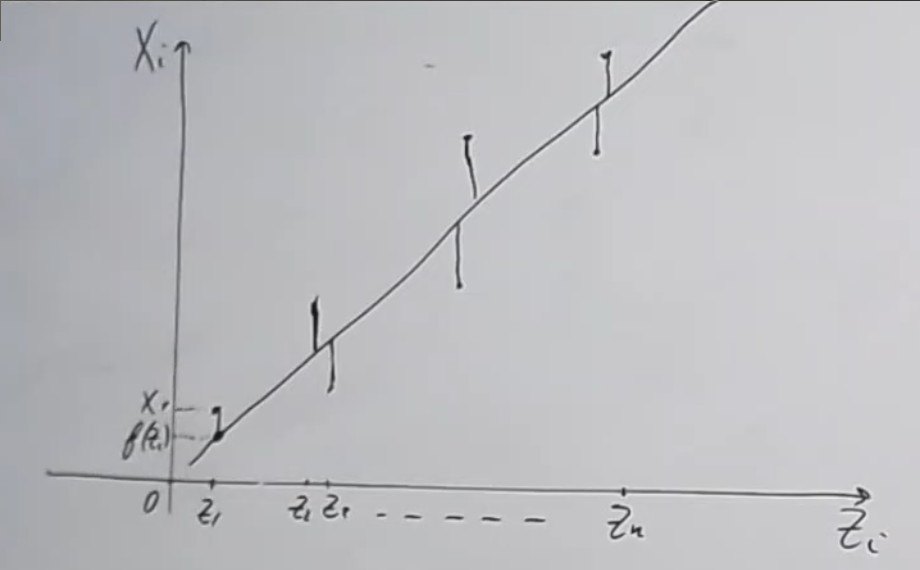
\includegraphics[scale=0.2]{imgs/regression.png}
\end{figure}

Прямая регрессии строится таким образом, чтобы сумма квадратов длин отрезков от прямой до точек распределения была наименьшей.
%</33>

\subsection{Выборочный коэффициент линейной корреляции}

%<*34>
\begin{definition}
    \begin{myemph}
        r_{\mathrm{в}} \coloneqq \frac{ \overline{XZ} - \overline{X} \cdot \overline{Z}}{ \hat{\sigma}_z \hat{\sigma}_x}
    \end{myemph}
\end{definition}

\begin{remark}
    Из прошлого семестра:
    \[r_{\xi, \eta} = \frac{\E \xi \eta - \E \xi \cdot \E \eta}{\sigma_\xi \cdot \sigma_\eta}\]
\end{remark}

Отсюда видим, что выборочный коэффициент линейной корреляции является оценкой теоретического коэффициента линейной корреляции, полученной по методу моментов. Поэтому выборочный коэффициент линейной корреляции характеризует силу линейной связи между двумя случайными величинами. Знак \(r_{\mathrm{в}}\) показывает, является ли корреляция прямой или обратной.

\begin{figure}[H]
    \centering
    \begin{tabular}{Ll}
        \toprule
        |r_{\mathrm{в}}| & Сила связи    \\ \midrule
        0.1-0.3          & слабая        \\
        0.3-0.5          & умеренная     \\
        0.5-0.7          & заметная      \\
        0.7-0.9          & высокая       \\
        >0.9             & очень высокая \\
        \bottomrule
    \end{tabular}
    \caption{Шкала Чеддока}
\end{figure}

\subsubsection{Проверка гипотезы о значимости выборочного коэффициента корреляции}

Пусть двумерная случайная величина \((Z, X)\) распределена нормально. По выборке объёма \(n\) вычислим \(r_{\mathrm{в}}\), а \(r\) --- теоретический коэффициент линейной корреляции. Проверяется основная гипотеза \(H_0 : r = 0\) против альтернативной гипотезы \(H_1 : r \neq 0\), т.е. коэффициент \(r_{\mathrm{в}}\) \underline{статистически значим}.

\begin{theorem}
    Если \(H_0\) верна, то статистика
    \[K = \frac{r_{\mathrm{в}} \sqrt{n - 2}}{\sqrt{1 - r_{\mathrm{в}^2}}} \in T_{n - 2}\]
\end{theorem}

Критерий: пусть \(t_k\) --- квантиль \(T_{n-2}\) уровня значимости \(\alpha\).
\[\begin{cases}
        H_0 : r = 0,    & |K| < t_k    \\
        H_1 : r \neq 0, & |K| \geq t_k
    \end{cases}\]
В Excel \(r_{\mathrm{в}} = \mathrm{КОРРЕЛ}(Z, X)\)
%</34>

\subsection{Исторический смысл понятия регрессии}

\unfinished

\begin{remark}\itemfix
    \begin{itemize}
        \item Из корреляции не следует зависимость.
        \item Зависимость и корреляция не транзитивны.
        \item Нулевая корреляция не гарантирует отсутствие зависимости
    \end{itemize}
\end{remark}

\subsection{Выборочное корреляционное отношение}

%<*35>
Пусть имеется \(k\) выборок случайной величины \(X\), полученных при уровнях фактора \(Z : Z_1 \dots Z_k\). Вычислены общая дисперсия \(D_o\), межгрупповая дисперсия \(D_{\mathrm{м}}\) и \(D_{\mathrm{в}}\) --- внутригрупповая дисперсия. По теореме \nameref{разложение дисперсий} \(D_o = D_{\mathrm{в}} + D_{\mathrm{м}}\). Обозначим:
\begin{itemize}
    \item \(\sigma_{ \overline{X}_z} = \sqrt{D_{\mathrm{м}}}\) --- межгрупповое среднеквадратическое отклонение
    \item \(\hat{\sigma}_X = \sqrt{D_{\mathrm{о}}}\) --- выборочное   среднеквадратическое отклонение
\end{itemize}

\begin{definition}
    \textbf{Выборочным корреляционным отношением} \(\eta_{XZ}\) случайной величины \(X\) на \(Z\) называется величина
    \begin{myemph}
        \eta_{XZ} = \frac{\sigma_{\overline{X}_z}}{\hat{\sigma}_X} = \sqrt{\frac{D_{\mathrm{м}}}{D_{\mathrm{о}}}}
    \end{myemph}
\end{definition}

\begin{prop}\itemfix
    \begin{enumerate}
        \item \(0 \leq \eta \leq 1\)
              \begin{proof}
                  \[D_o = D_{\mathrm{в}} + D_{\mathrm{м}}, 0 \leq D_{\mathrm{м}} \leq D_o \Rightarrow 0 \leq \frac{D_{\mathrm{м}}}{D_o} \leq 1 \Rightarrow 0 \leq \eta = \sqrt{\frac{D_{\mathrm{м}}}{D_o}} \leq 1\]
              \end{proof}
        \item Если \(\eta = 1\), то \(X\) функционально зависит от \(Z\).
              \begin{proof}
                  \(\eta = 1 \Rightarrow D_{\mathrm{в}} = 0 \Rightarrow X = X(Z)\) --- функция от переменной \(Z\)
              \end{proof}
        \item Если \(\eta = 0\), то нет корреляционной зависимости.
              \begin{proof}
                  Если \(\eta = 0\), то \(D_{\mathrm{м}} = 0\), следовательно значения \(\overline{X}^{(i)}\) не зависят от \(Z_i\).
              \end{proof}
        \item \(\eta \geq |r_{\mathrm{в}}|\)
        \item \(\eta = |r_{\mathrm{в}}| \Leftrightarrow \) когда имеет место точная линейная корреляционная зависимость, т.е. все точки экспериментальных данных лежат на одной прямой, которая совпадёт с прямой регрессии.
    \end{enumerate}
\end{prop}
%</35>
